\section{Background}
\begin{frame}{\secname}
	\framesubtitle{Power Systems}
	\begin{columns}
	\begin{column}{0.5\textwidth}
		\begin{itemize}
			\item<1-> Large interconnected system
			\item<2-> Balancing challenge
		\end{itemize}
	\end{column}
	\begin{column}{0.5\textwidth}	
	\begin{figure}
	\begin{center}
	\includegraphics<1>[width=0.7\textwidth]{./pictures/nordic}
	\caption{Nordic power system[ENTSO-e]}
	\includegraphics<2->[width=0.7\textwidth]{./pictures/balance}
	\caption{Balancing challenge[Statnett]}
	\end{center}
	\end{figure}
	\end{column}
	\end{columns}
\end{frame}
\begin{frame}{\secname}
	\framesubtitle{Challenges in operation}
	\begin{columns}
		\begin{column}{0.5\textwidth}
		\begin{itemize}
			\item<1-> Towards 100\% renewable electricity generation
			\begin{itemize}
				\item Larger variability
				\item More uncertainty
				\item Increasing complexity
			\end{itemize}
			\item<2-> More dynamics
			\item<3-> Less time for actions
			\item<4-> \textbf{Hydropower} is the main resource for balancing
\end{itemize}
\end{column}
	\begin{column}{0.5\textwidth}
	\begin{figure}
	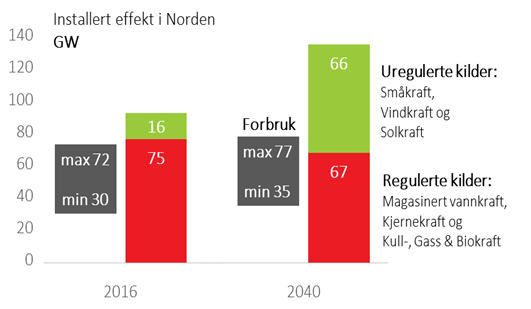
\includegraphics[width=0.8\textwidth]{./pictures/mix}
	\caption{Present and future energy mix[Statnett]}
	\end{figure}
	\end{column}
	\end{columns}
\end{frame}
\begin{frame}{\secname}
	\framesubtitle{Frequency containment reserves (FCR)}
	\begin{columns}
		\begin{column}{0.5\textwidth}
			\begin{itemize}
				\item<1-> Power balance/frequency containment control (FCC) is mainly determined by governor response.
				\item<1-> Activation of primary reserves is determined by the governor droop settings.
				\item<2-> In steady state
			\end{itemize}
		\end{column}
		\begin{column}{0.5\textwidth}	
			\begin{figure}
					\includegraphics[width=\textwidth]{./pictures/speedDroop.tikz}
			\end{figure}
		\end{column}
	\end{columns}
\end{frame}
\begin{frame}{\secname}
	\framesubtitle{The power system is dynamic}
	\begin{figure}
		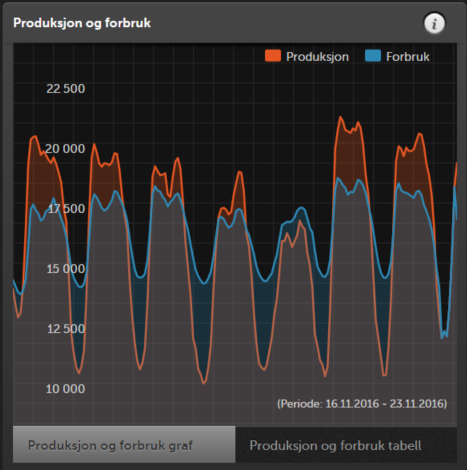
\includegraphics[width=0.5\textwidth]{./pictures/static}
		\caption{Production and consumption [statnett.no]}
	\end{figure}
\end{frame}
\begin{frame}{\secname}
	\framesubtitle{Frequency quality in the Nordics}
	\begin{columns}
		\begin{column}{0.5\textwidth}
			\begin{itemize}
				\item From 2008 the time the frequency has been outside its allowed band has increased
				\item The performance of hydro turbine governors play an important role
			\end{itemize}
		\end{column}
		\begin{column}{0.5\textwidth}
			\begin{figure}
				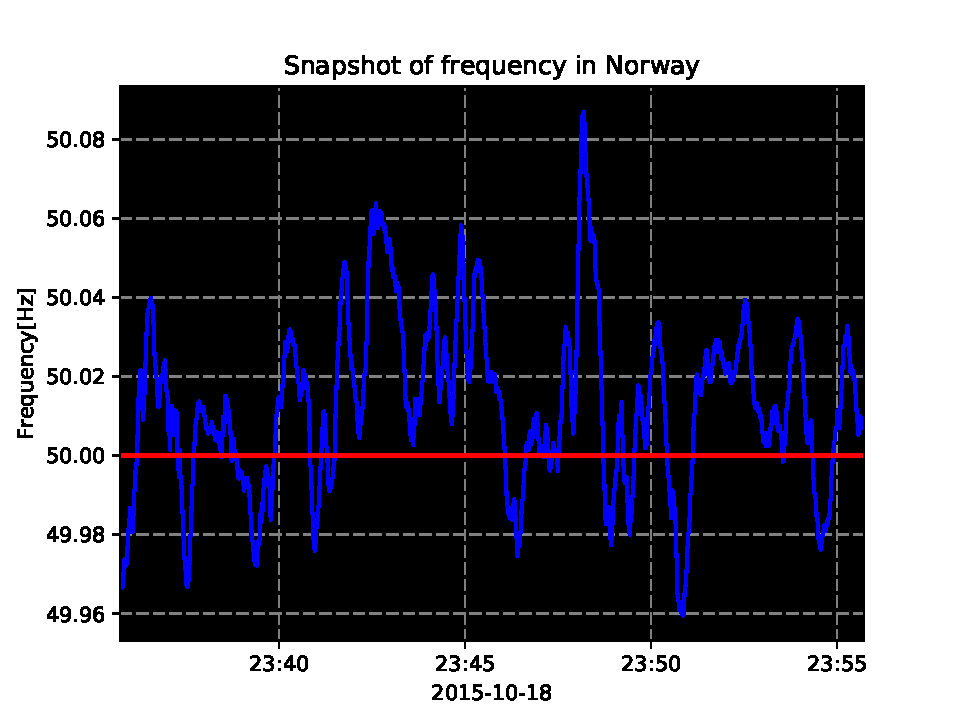
\includegraphics[width=0.8\textwidth]{./pictures/frequency.pdf}
			\end{figure}
		\end{column}
	\end{columns}
\end{frame}
\begin{frame}{\secname}
	\framesubtitle{New requirements on FCR}
	\begin{itemize}
		\item Nordic TSOs are developing new requirements on FCR
		\item This includes offline testing and verification of performance
		\begin{figure}
				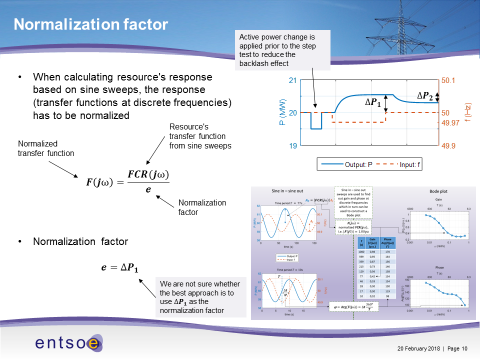
\includegraphics[width=0.4\textwidth]{./pictures/fcr}
		\end{figure}
	\end{itemize}
\end{frame}
\begin{frame}{\secname}
	\framesubtitle{Research question}
	\begin{enumerate}
		\item<1-> Do the transmission system operator (TSO) know whether or not the hydropower plants deliver the FCR they are supposed to?
		\item<2-> Can the measure it online?
	\end{enumerate}
\end{frame}
